\section{Problemstellung und Requirements}
\label{sec-3}
\begin{center}
	\fbox{
		\parbox{0.9\linewidth}{
			\textit{Ziel des Kapitels:}\\
			Anforderungen von technischer und anwendungsorientierter Seite darstellen und Problem formulieren.
	}}\\
\end{center}

%Auf Basis der Hintergrundinformationen aus dem vorangegangenen Kapitel können nun konkrete Probleme identifiziert und formuliert werden. 

Einleitung

%TODO formulierungen überarbeiten
\begin{comment}
Ziel dieser Arbeit ist am konkreten Beispiel der Helmholtz-Spule zu untersuchen, wie die HoloLens in der Physik Lehre eingesetzt werden kann. Dazu betrachtet die Arbeit speziell, wie der zuvor beschriebene Versuchsaufbau mit Informationen angereichert werden kann. Aufbauend auf den im vorigen Kapiteln erarbeiteten Hintergründen formulieren die folgenden Abschnitte an die Anwendung zu stellende Anforderungen aus anwendungsorientierter sowie technischer Sicht.\\

Wie kann die HoloLens für diesen Versuch konkret eingesetzt werden?\\
\end{comment}

\begin{figure}[h!]
	\centering
	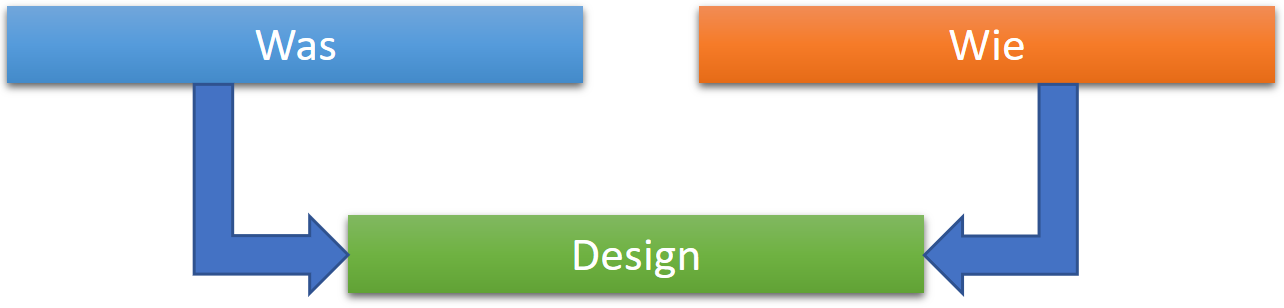
\includegraphics[width=0.6\textwidth]{images/Informiertes_Design.png}
	\caption{Informiertes Design}
	\label{img:Informiertes_Design}
\end{figure}

\subsection{Anforderungen}
\label{sec-3-1}
%TODO formulierungen überarbeiten
Die Anforderungen an eine Umsetzung kommen aus zwei Bereichen: Zum einen aus der Physik und zum anderen aus den technischen Modalitäten der HoloLens. Ein Design muss beide berücksichtigen und zusammenführen zu einer Lösung. Dabei bestimmt das Anwendungsszenario vor allem die inhaltlichen Anforderungen während die technischen Gegebenheiten eher auf das ''Wie'' der Umsetzung Einfluss nehmen. Zunächst sollen die inhaltlichen Anforderungen aufgestellt werden.

\subsubsection{Was - Physik}
Zunächst stellt sich die Frage, welche Informationen zum Versuchsaufbau über die Anwendung integriert werden sollen. Von besonderem Interesse sind hier natürlich vor allem Informationen, die für den Nutzer nicht direkt beobachtbar sind. Das betrifft in erster Linie die beiden sich überlagernden Magnetfelder von Erde und Spule mit deren Eigenschaften. Das Zusammenspiel beider Felder ist elementar für den Versuch und soll für den Anwender sichtbar gemacht werden. Weitere, nicht direkt erkennbare Eigenschaften  des Versuches sind außerdem wie die Richtung des Stromflusses durch die Spule und die physikalischen Parameter des Versuchsaufbaus.\\

Ein weiterer interessanter Aspekt ist die Einbindung theoretischer Ergebnisse. Das ermöglicht dem Anwender direkt am Versuchsaufbau sowohl gemessene als auch berechnete Werte zu erfassen und beide miteinander zu vergleichen. Bei der Bestimmung des Erdmagnetfeldes betrifft das vor allem die Auslenkung des Kompasses, die sich in Abhängigkeit der anliegenden Stromstärke verändert. Die Magnetnadel des Kompass unterliegt dabei Faktoren wie Reibung und Trägheit, die zu Abweichungen führen können. Ein berechneter, virtueller Kompass unterliegt solchen Einschränkungen nicht und kann ergänzend zum realen Konterpart das angenommene Verhalten des Systems unter Idealbedingungen aufzeigen.\\

Unter diesen Gesichtspunkten und für den Rahmen dieser Arbeit wurden in Zusammenarbeit mit Physikern die folgenden Anforderungen im Hinblick auf die darzustellenden Elemente aufgestellt:\\[4px]
\textbf{Funktionale Anforderungen}
\begin{enumerate}[topsep=-2px]
	\setlength{\itemsep}{-5pt}
	\item Magnetfeld von Erde und Spule
	\begin{itemize}[topsep=-0.25em]
		\setlength{\itemsep}{-0.25em}
		\item Stärke
		\item Richtung
		\item Homogenität
		\item Inhomogenität am Rand der Spule andeuten (Optional) 
	\end{itemize}
	\item Stromfluss durch die Spule
	\begin{itemize}[topsep=-0.25em]
		\setlength{\itemsep}{-0.25em}
		\item Richtung
		\item Kennzeichnung von Plus und Minus
		\item Stärke (Optional) 
	\end{itemize}
	\item Kompass
	\begin{itemize}[topsep=-0.25em]
		\setlength{\itemsep}{-0.25em}
		\item Nordrichtung
		\item Grobe Auslenkung der Nadel
	\end{itemize}
	\item Weitere Informationen (Optional)
	\begin{itemize}[topsep=-0.25em]
		\setlength{\itemsep}{-0.25em}
		\item Windungszahl der Spule
		\item Durchmesser und Abstand der Spulen
		\item Numerische Werte und Informationen (z.B. Fließt aktuell Strom, angelegte Stromstärke, angenommene Stärke des Erdmagnetfeldes, systematischer und zufälliger Fehler, etc.)
	\end{itemize}
\end{enumerate}

Diese Anforderung verlangen dabei nicht notwendigerweise (rein) virtuelle Repräsentationen für die genannten Elemente. Auch wenn der Fokus auf über die HoloLens visualisierten Daten liegt, so könnte es für manche Elemente sinnvoller sein auf andere Optionen zurückzugreifen. Das können reale statt virtueller Objekte sein aber auch akustische Informationen, die über die integrierten Lautsprecher der HoloLens wiedergegeben werden. Die Frage, was visualisiert und auch was nicht visualisiert wird, ist also durch ein Design zu beantworten.\\

Neben diesen eher funktionalen Anforderungen sind von Seiten der Physik auch nicht-funktionale Anforderungen an die Anwendung zu stellen. Hier wurden die Folgenden herausgearbeitet:\\[4px]
\textbf{Nicht-funktionale Anfoderungen}
\begin{itemize}[topsep=-2px]
	\setlength{\itemsep}{-5pt}
	\item Darstellungen müssen physikalisch korrekt und interpretierbar sein
	\item Nutzer darf nicht in seiner Interaktion mit dem Versuchsaufbau und relevanten Materialien eingeschränkt werden
	\item Anwendung sollte auch für Nutzer ohne Erfahrung mit der HoloLens nutzbar sein
	\item Die vorhandenen Lehrmittel sollten genutzt werden
\end{itemize}
\vspace{4px}
Der erste Punkt soll hier kurz näher beleuchtet werden. Dabei geht es nicht um möglichst exakte Werte und Darstellungen. Vielmehr sollen sie physikalisch interpretierbar sein, indem auf etablierte Modelle zurückgegriffen wird. Außerdem sollen sie keine falschen Eindrücke vermitteln und die physikalischen Zusammenhänge korrekt widerspiegeln.\\

\subsubsection{Wie - Technische Seite}
In Kapitel \ref{sec-2-1} wurde die HoloLens mit ihren technischen Möglichkeiten aber auch Einschränkungen vorgestellt sowie Auswirkungen auf das Anwendungsdesign aufgezeigt. Die genannten Probleme sollen möglichst vermieden werden, indem die Anwendung an die speziellen Gegebenheiten der HoloLens angepasst wird. Dementsprechend sollen auch von technischer Seite Anforderungen aufgestellt werden.\\

Die Dokumentation zu Windows Mixed Reality enthält eine Liste von Qualitätskriterien, anhand derer Anwendungen bewertet werden können. Diese deckt viele der zuvor erläuterten Probleme wie z.B. der Abstand zu Objekten ab. Jedes Kriterium ist mit einer Beschreibung versehen, unter welchen Umständen es als optimal erfüllt, erfüllt oder nicht erfüllt gilt. Eine Kurzfassung relevanter Kriterien ist in Tabelle \ref{tab:tech_criteria} zusammengestellt.\\

\bgroup
\setlength\extrarowheight{-2pt}
\def\arraystretch{2}
\begin{table}[htb]
	\centering
	\begin{tabular}{l|l}
		Kriterium & Kurzbeschreibung \\
		\hline
		Framerate & Gibt die Anwendung konstant 60 FPS aus?\\
		Stabilität der Hologramme & Weisen Hologramme bei Bewegungen Ruckler, Sprünge, Drift, Wackeln, Wippen oder ähnliches auf?\\
		Positionierung & Sind Hologramme im Verhältnis zu realen Objekten korrekt positioniert?\\
		Komfortzone & Liegen Distanz und Betrachtungswinkel in den empfohlenen Bereichen?\\
		Tiefen Wechsel & Bedingt die Anwendung häufige Fokuswechsel?\\
		FOV-Grenzen & Behindern die Begrenzungen des FOV die Nutzererfahrungen?\\
		Input Interaction Clarity & Werden konsistente, bekannte und geeignete Eingabemethoden geboten?\\
		Anpassung an Nutzerposition & Passen sich Darstellungen der Position des Nutzers an?\\
		Interaktive Objekte & Sind interaktive Objekte als solche erkennbar?\\
		Ladevorgänge  & Erhält der Nutzer Feedback über länger laufende Operationen?\\
	\end{tabular}\caption{\label{tab:tech_criteria} Kurzfassung der Qualitätskriterien.}
\end{table}
\egroup

An diesen Kriterien soll sich die Lösung orientieren und diese bereits im Design berücksichtigen. Dafür sollen die genannten Hinweise und Empfehlungen zum Design mit einbezogen und darauf aufgebaut werden.\\

\subsection{Problemstellung}
\label{sec-3-2}
Die inhaltlichen und technischen Anforderungen stecken den Rahmen ab, für den eine Lösung zu erarbeiten ist. Dazu ist ein Design nötig, dass die inhaltlichen Anforderungen bedient, dabei die Möglichkeiten der HoloLens nutzt und gleichzeitig um technische Einschränkungen und Besonderheiten herum navigiert.\\

Eine Lösung muss die folgenden Fragen beantworten:
\begin{itemize}
	\setlength{\itemsep}{-5pt}
	\item Was soll dargestellt werden? (Was soll nicht dargestellt werden?)
	\item Wie soll es dargestellt werden?
	\item Wie soll damit interagiert werden?
\end{itemize}

\textbf{\textit{Was soll dargestellt werden?}}\\
Zunächst stellt sich die Frage, welche Objekte die HoloLens zusätzlich anzeigen soll. Hier geben die funktionalen Anforderungen bereits einige Elemente vor, die weiter konkretisiert werden müssen. Hier stellt sich auch die Frage, welche Informationen über reale Objekte (wie z.B. digitales Amperemeter) transportiert und nicht über die HoloLens dargestellt werden sollen. Bei diesen und ggf. weiteren Objekten ist beim Design zu berücksichtigen, dass sie durch virtuelle Darstellungen nur bedingt überblendet werden sollten.\\

Dazu kommen als optional eingestufte Elemente sowie Informationen, die den Ablauf und die Interaktion mit der Anwendung betreffen. Das betrifft z.B. Feedback für Nutzeraktionen, den Cursor oder Statusinformationen.\\

\textbf{\textit{Wie soll es dargestellt werden?}}\\
Die wohl umfassendste Frage besteht darin, wie die Informationen und Zusammenhänge visualisiert werden sollen. Was soll textuell, als 2D oder als 3D Geometrie dargestellt werden? \\

\textbf{\textit{Wie soll damit interagiert werden?}}\\
Nicht zuletzt ist ein Konzept für die Interaktion zu erstellen. Welche Eingabemethoden werden dem Nutzer angeboten und wie wird der Nutzer über diese informiert? Welche Aktionen soll die Anwendung zur Verfügung stellen?\\

